%\documentclass[landscape,a0b,final,a4resizeable]{a0poster}
% \documentclass[landscape,a0b,final]{a0poster}
\documentclass[landscape,a0b,final]{a0poster}
%\setlength{\paperwidth}{48in}
%\setlength{\paperheight}{36in}
%\setlength{\textwidth}{20in}
%\setlength{\textheight}{50in}

%\setlength{\textwidth}{15in}
%\setlength{\textheight}{20in} 
% \documentclass[portrait,a0b,final,a4resizeable]{a0poster}
% \documentclass[portrait,a0b,final]{a0poster}
%%% Option "a4resizeable" makes it possible ot resize the
% poster by the command: psresize -pa4 poster.ps poster-a4.ps
% For final printing, please remove option "a4resizeable" !!

%\usepackage{epsfig}
\usepackage{multicol}                                           %Multiple Columns
\usepackage[left=1cm,right=1cm,bottom=1cm,top=1cm]{geometry}	%Reset margins
\usepackage{times,amsmath,float,color}
\usepackage{graphicx} 
\usepackage{hhline}
\usepackage{natbib}
\usepackage[T1]{fontenc}			%Need for gtamac fonts
\usepackage{textcomp}
\usepackage{mathpazo}			%Load palatino font & pazo math
\usepackage{times}
\usepackage{wrapfig}
\bibliographystyle{/Users/hpm/D_DRIVE/latex/agu} 
%\usepackage{tabular}
%\usepackage[large]{subfigure} 
%\usepackage[latin1]{inputenc}
%\usepackage[font=scriptsize,bf]{caption}
\DeclareGraphicsRule{.tif}{png}{.png}{`convert #1 `dirname #1`/`basename #1 .tif`.png}

\def\sA{{\mathcal{A}}}
\def\sB{{\mathcal{B}}}

%%%%%%%%%%%%%%%%%%%%%%%%%%%%%%%%%%%%%%%%%%% 
% Definition of some variables and colors
%%%%%%%%%%%%%%%%%%%%%%%%%%%%%%%%%%%%%%%%%%

% \renewcommand{\rho}{\varrho}
% \renewcommand{\phi}{\varphi}
\setlength{\columnsep}{3cm}                     %Set spacing between columns
\setlength{\columnseprule}{2mm}                 %lines as column separators
\setlength{\parindent}{0.0cm}

%%%Define colours and lengths
\definecolor{headingcol}{rgb}{1,0.7,0}		%Color of main title
\definecolor{fillcol}{rgb}{0.9,0.9,1}	        %Fill-color of box
\definecolor{boxcol}{rgb}{0.2,0.2,0.5}		%Edge-color of box and top banner
\fboxsep=0.5cm					%Padding between box and text
\fboxrule=1.5mm					%Width of box outline
\renewcommand{\rmdefault}{ppl}			%Reset serif to Palatino

% Figures within a column:
\makeatletter
\newenvironment{tablehere}
{\def\@captype{table}}
{}
\newenvironment{figurehere}
{\def\@captype{figure}}
{}
\makeatother

% changing the font of the caption, to make it stick out
%\usepackage[font=sf]{caption}
%\setlength{\belowcaptionskip}{15pt}

%%% Format title
\makeatletter				%Needed to include code in main file
\renewcommand\@maketitle{%
\null					%Sets position marker
{
\color{headingcol}\sffamily\veryHuge	%Set title font and color (from above)
\@title \par}%
\vskip 0.6em%
{
\color{white}\sffamily\large		%Set author font and color(white)
\lineskip .5em%
\begin{tabular}[t]{l}%
\@author
\end{tabular}\par}%
\vskip 1cm
\par
}
\makeatother

\newsavebox\envbox 			%Define name for boxes used

%%%%%%%%%%%%%%%%%%%%%%%%%%%%%%%%%%%%%%%%%%%%%%%%%%
%%% Define "Section" environment for framed boxes
%%% Usage: \begin{Section}{Name} blah blah blah \end{Section}
%%%%%%%%%%%%%%%%%%%%%%%%%%%%%%%%%%%%%%%%%%%%%%%%%

\newenvironment{sectionbox}[1]		%Environment takes one argument
%%%Opening
{
\par 
\flushleft
\colorbox{boxcol}{ 				%Draws solid color box around title
\sffamily\Large \color{white} #1                %Typesets section name
\hspace{0.5cm}}
\par\nobreak 
\nointerlineskip 				%Fits title snugly above box (no gap)
\setlength\parskip{-1pt}			%Even snugger
\begin{lrbox}\envbox				%Opens box environment
\begin{minipage}{0.9\columnwidth}		%Opens minipage environment for section contents
}
%%%Closing
{\par
\end{minipage}\end{lrbox}			%Close minipage and box
\fcolorbox{boxcol}{fillcol}{\usebox\envbox}	%Draw box with contents frame color: boxcol, fill color: fillcol
\vspace{1cm}					%Add spacing below box
} 

%%% This will just create a section title with no box but with horizontal line
\newenvironment{mysection}[1]		%Environment takes one argument
%%%Opening
{
\vspace{\fboxsep}                                    %Create space between area above
\par
\colorbox{boxcol}{ 				%Draws solid color box around title
\sffamily\Large \color{white} #1                %Typesets section name
\hspace{0.5cm}}
\par\nobreak 
\nointerlineskip 				%Fits title snugly above box (no gap)
\vspace{-\fboxsep}
{\color{boxcol}\rule{1\linewidth}{\fboxrule}}
\vspace{\fboxsep}                                 %Space below line and text
}


%%%%%%%%%%%%%%%%%%%%%%%
%%% Poster                                       %%%
%%%%%%%%%%%%%%%%%%%%%%%
% create a poster size that is just smaller than the
% text width to ensure the margins
\newenvironment{poster}{
  \begin{center}
    \begin{minipage}[c]{0.98\textwidth}
    }{
    \end{minipage} 
  \end{center}
}

%%%%%%%%%%%%%%%%%%%%%%%%%
%%% symbols for author affiliations              %%%
%%%%%%%%%%%%%%%%%%%%%%%%%     
\def\thefootnote{\fnsymbol{footnote}}

%%%%%%%%%%%%%%%%%%%%%%%%%
%%% Add authors and affiliations                %%%
%%%%%%%%%%%%%%%%%%%%%%%%%
 
\title{\begin{center} C15G-0877 - Observations of depth, SWE, and stratigraphy using FMCW radar and machine learning, during the NASA SnowEx 2020 Grand Mesa Campaign \end{center} }
% \vspace{0.5cm}
\author{ \LARGE{Hans-Peter Marshall$^{1*}$, Scott Storms$^{1,2}$, Eli Deeb$^2$, Carrie Vuyovich$^3$, Kelly Elder$^4$, Mike Durand$^5$} \\ % \vspace{0.2cm}
\textbf{1} \textit{Cryosphere Geophysics And Remote Sensing (CryoGARS) lab and Department of Geosciences, Boise State University} \\
\textbf{2} \textit{U.S. Army Cold Regions Research and Engineering Laboratory} \\
\textbf{3} \textit{Goddard Space Flight Center} \\
\textbf{4} \textit{USFS Rocky Mountain Research Center, Fraser Experimental Forest} \\
\textbf{5} \textit{The Ohio State University, Byrd Polar Research Center}
%\textbf{3} \textit{USFS Rocky Mountain Research Station, Fraser Experimental Forest and Ft. Collins, Colorado} 
%\textbf{4} \textit{NASA Jet Propulsion Laboratory} \\
\textbf{*} \textit{email: hpmarshall@boisestate.edu, earth.boisestate.edu/cryogars}}

%, , \\
%}}
%\vspace{0.5cm}
%\textbf{1} Center for Geophysical Investigations of the Shallow Subsurface, Boise State University, Boise, ID, USA}
%\title{{\bf C31A-0600:}Inversion of FMCW radar with a priori information from SMP measurements\vspace{0.5cm}}
%\author{\LARGE{Scott Havens\footnotemark[1], Hans-Peter Marshall\footnotemark[1], and John Bradford\footnotemark[1]}\\
%\Large{\footnotemark[1] \hspace{3mm} Center for Geophysical Investigations of the Shallow Subsurface, Boise State University, Boise, ID, USA}}


%%%%%%%%%%%%%%%%%%%%%%%%%%%%%%%%%%%%%%%%%%
%%% Begin of Document
%%%%%%%%%%%%%%%%%%%%%%%%%%%%%%%%%%%%%%%%%%

\begin{document}

\floatplacement{figure}{H} 

%\hspace{-2cm}			%Align with edge of page, not margin
\colorbox{boxcol}{		%Colored banner across top
\begin{minipage}[c]{0.80\textwidth}	%Minipage for title contents
%\vspace{-3cm}			%Shift up over header image
\maketitle
\end{minipage}

% Right logos
\begin{minipage}[c]{0.20\textwidth}
\begin{flushright}

\includegraphics[height=5.5cm]{SnowExLogo.png} \vspace{0.2cm}

\includegraphics[height=5.5cm]{CRRELlogo.png} \hspace{0.2cm} 
\includegraphics[height=5.5cm]{USFS_RMRS_logo.png} \hspace{0.2cm} \\

\includegraphics[height=5.5cm]{NASA.pdf} \vspace{0.6cm} 
\includegraphics[height=5.5cm]{GSFC_logo.jpeg} \hspace{0.2cm} 

\includegraphics[height=5.5cm]{OSUlogo.jpeg} \\

\includegraphics[height=5.5cm]{BSU.png} \hspace{0.2cm} 
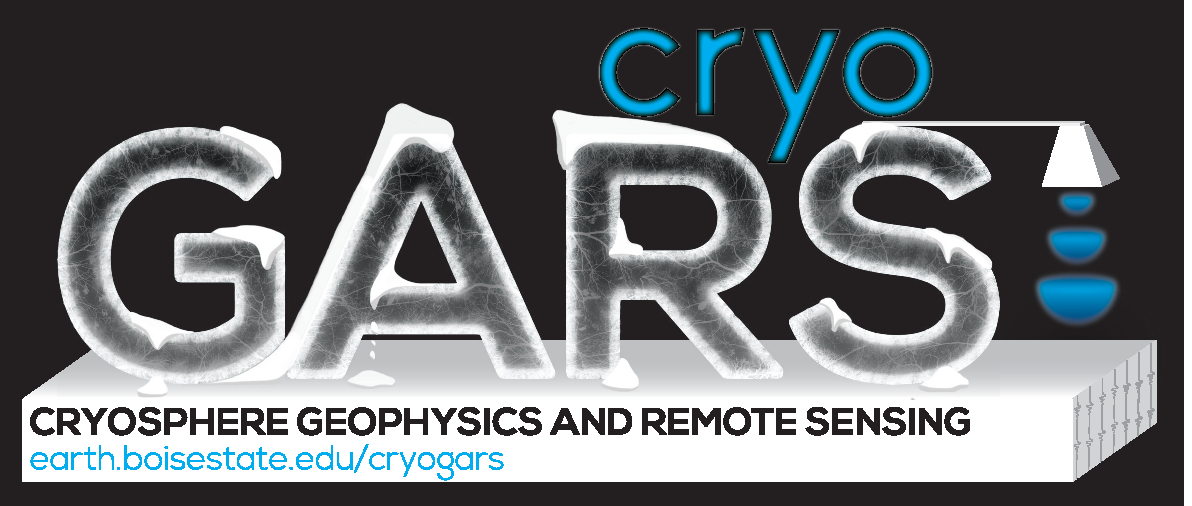
\includegraphics[height=6cm]{CryoGARSlogo.eps} \\

\end{flushright}
\end{minipage}

}
\vspace{1cm}

\begin{poster}
\thispagestyle{empty}
\begin{multicols}{4}		%Use 4-column layout
%\raggedcolumns			%Don't stretch contents vertically
%\raggedbottom

%%%%%%%%%%%%%%%%%%%%% 
%%% Content
%%%%%%%%%%%%%%%%%%%%% 
  
\begin{sectionbox}{Abstract}
\normalsize{Snow properties can vary significantly over distances of 50-200 meters, and therefore rapid techniques for measuring bulk snow properties are valuable for calibration and validation of snow remote sensing efforts. We developed and deployed a ground-based microwave radar from a snowmobile, during a large NASA snow remote sensing campaign. These observations provide information about the spatial distribution of snow depth, snow water equivalent, and stratigraphy, and were performed coincident with many different airborne snow remote sensing observations.}

%We performed ground-based Frequency Modulated Continuous Wave (FMCW) radar surveys during the 3 week NASA SnowEx 2020 Grand Mesa Intensive Observation Period (IOP). FMCW radar at microwave frequencies can be used to estimate snow depth, snow water equivalent, and is sensitive to stratigraphy. These observations can be made rapidly (100 Hz), and by deploying this system on a snowmobile, we mapped snow conditions between and around over 100 snowpits during this campaign. These observations provide information about how snow conditions change between validation manual snowpits, and can be used to quantify the variability at the 100 meter scale around each pit. However, interpretation can be time consuming, as typically layer interfaces require manual picking. We use a genetic algorithm and a neural network to automatically identify the surface and ground reflections, which enables automated inversion for bulk snow properties. Our radar system has been developed at Boise State University, covers a frequency range of 6-18 GHz, is dual polarization, and was deployed at nadir incidence angle. These observations were made on almost every day of the 3-week IOP, coincident with 5 different aircraft that deployed 7 different airborne instruments. Measurements at X and Ku bands provide not only information about the spatial distribution of bulk snow properties, but also allow insight into the impact of layering on microwave radar observations, at the frequencies currently targeted for spaceborne snow observations.

\end{sectionbox}

\begin{figure}
\centering
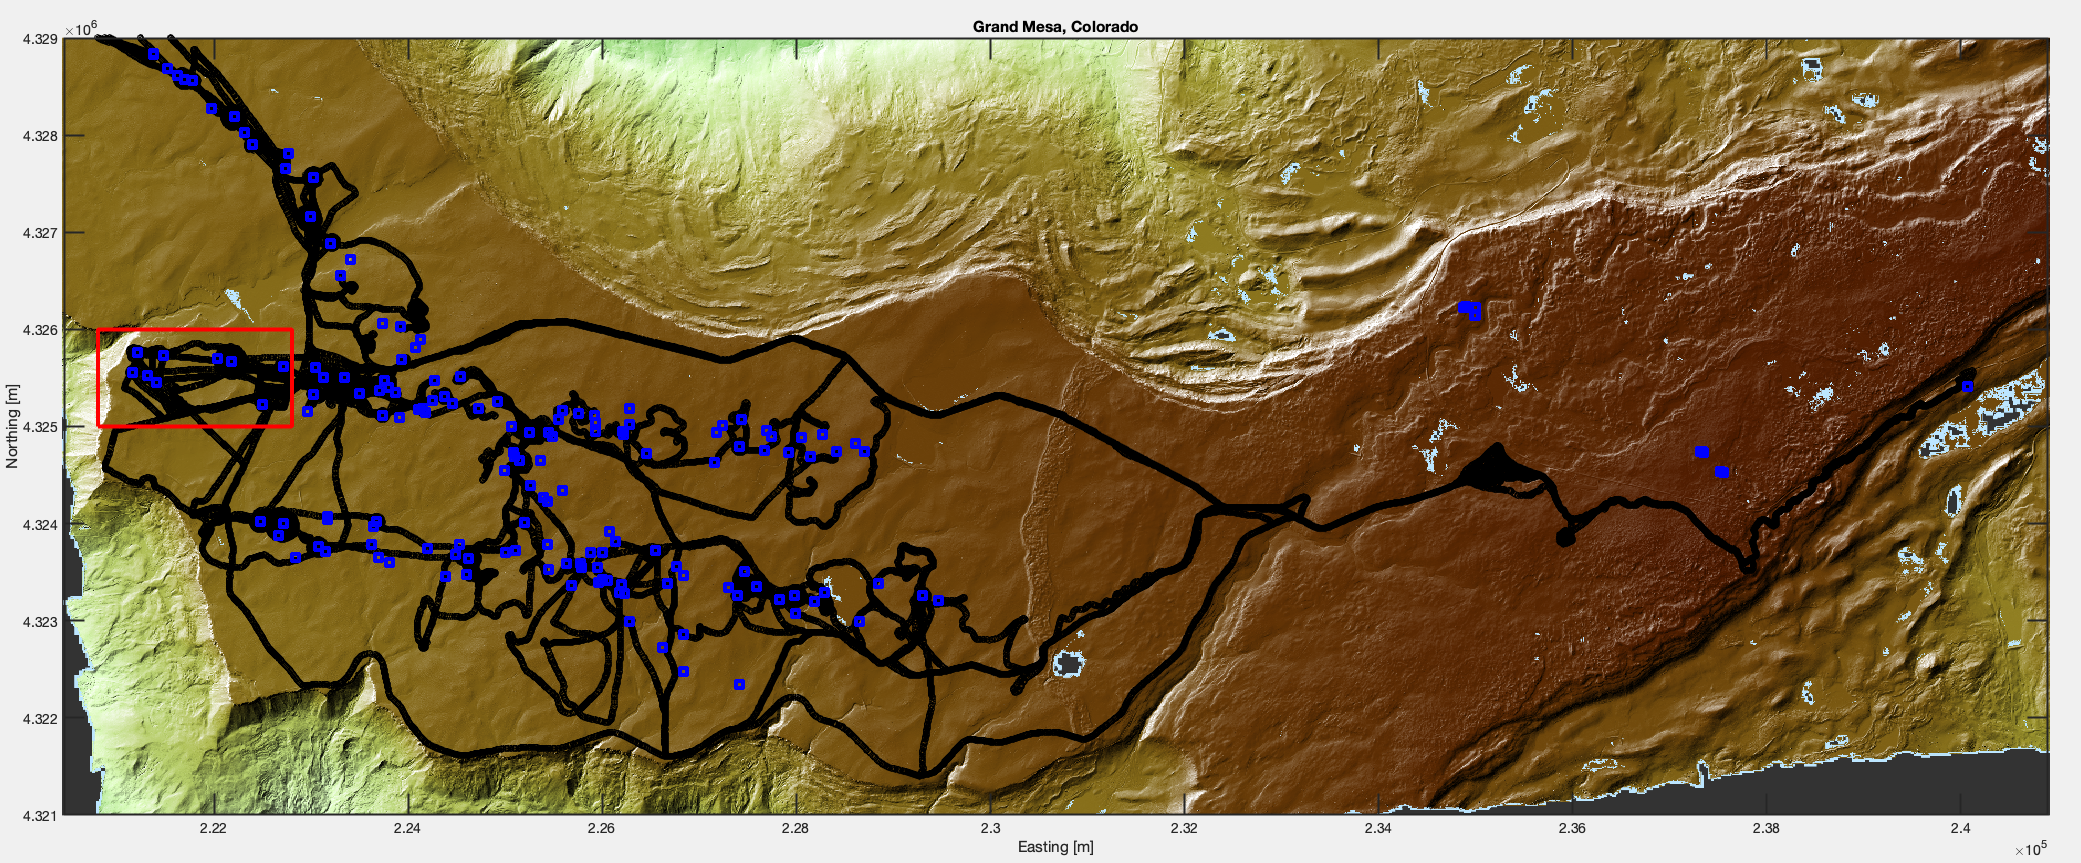
\includegraphics[width=1\columnwidth]{FIGURES/FMCWmap3.png}
\caption{Map of Grand Mesa with radar profiles (black), and snowpits (blue), over a 20km x 8km region.  Red box shows 2km x 1km area below.}
\label{fig:ProfileTrace} 
\end{figure}

\begin{figure}
\centering
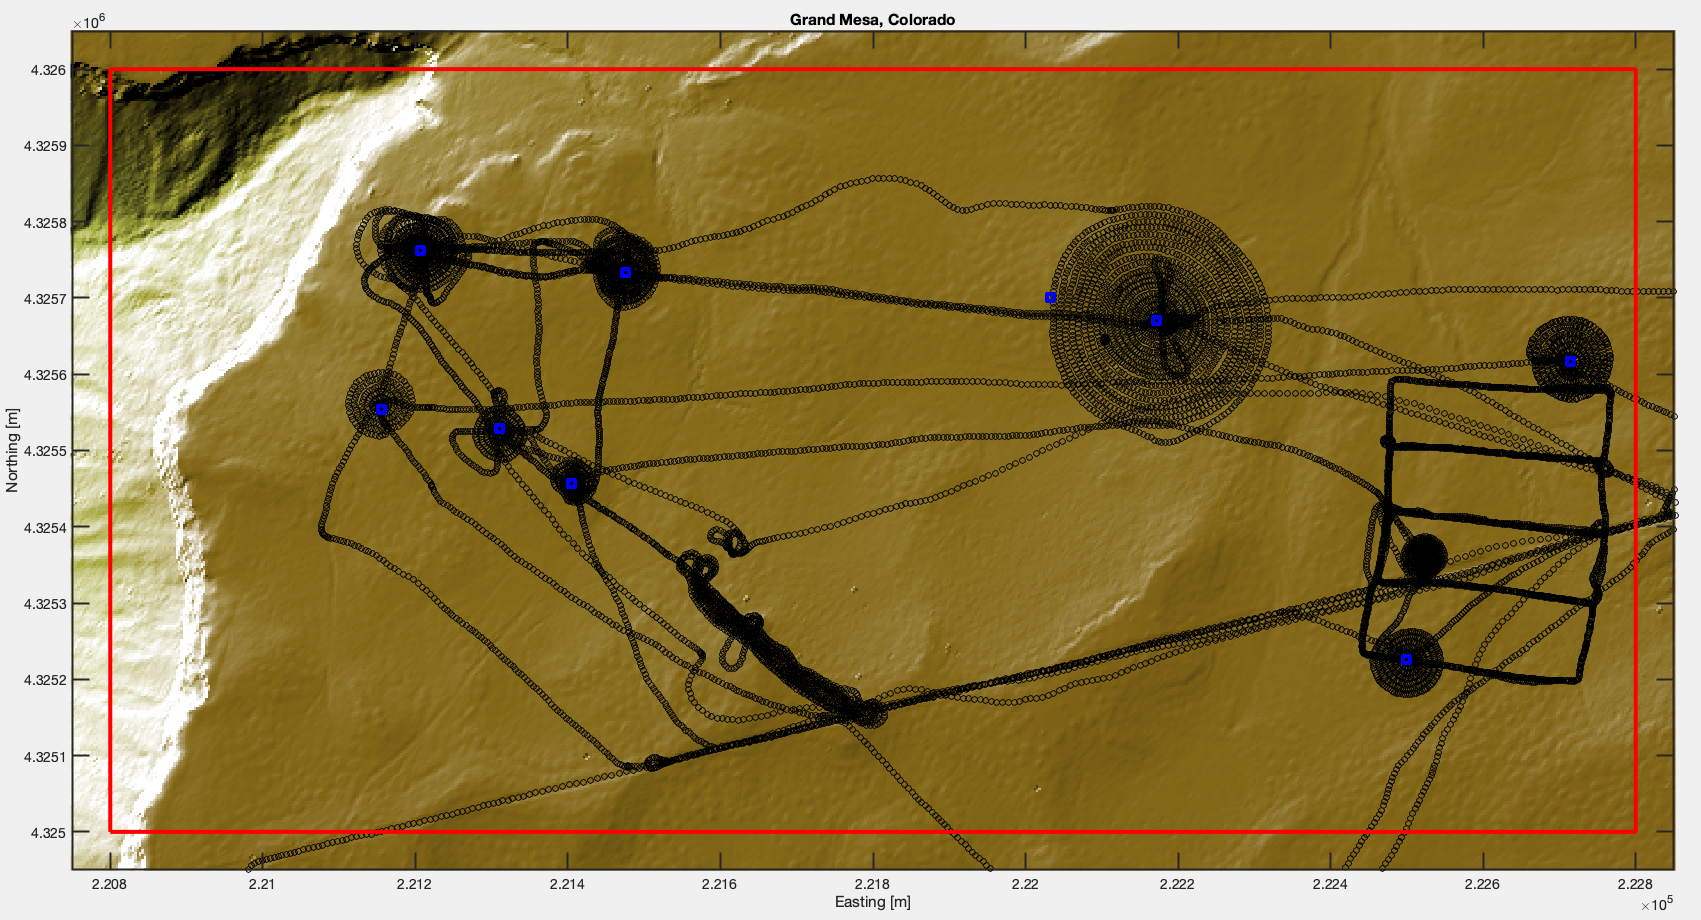
\includegraphics[width=1\columnwidth]{FIGURES/FMCWmap4.png}
\caption{Grand Mesa map zoomed in to red box (2km x 1km) in figure above, to show different radar sampling strategies.}
\label{fig:ProfileTrace} 
\end{figure}


\begin{mysection}{Introduction}
\vspace{-1cm}
\large{
\begin{itemize}
\item FMCW radar profiles during nearly all field sampling days of the SnowEx 2020 Grand Mesa IOP \citep[e.g.][]{Marshall:2008}
\item FMCW radar surveys sampled snow conditions near almost all 150+ SnowEx pits
\item Manual layer picking of surface and  ground returns represents the bottleneck in this massive dataset
\end{itemize}

\begin{minipage}{1\columnwidth}
\begin{figure}
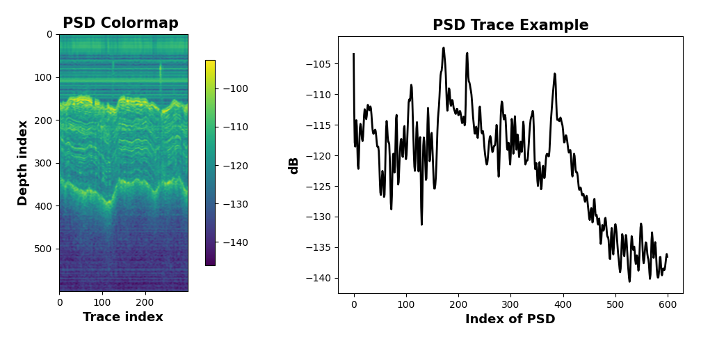
\includegraphics[width=1.05\columnwidth]{FIGURES/ProfileTrace.png}
\caption{Example FMCW profile (left) and an individual trace (right)}
\label{fig:ProfileTrace} 
\end{figure}
\end{minipage}

}
\end{mysection}

\begin{mysection}{Radar processing}
\large{
\begin{itemize}
\item Time domain signal is converted to frequency domain using FFT and Kaiser-Bessel window
\item Frequent sky calibration measurements used to remove instrumentation noise
\end{itemize}


\begin{minipage}{1.05\columnwidth}
\begin{figure}
\centering
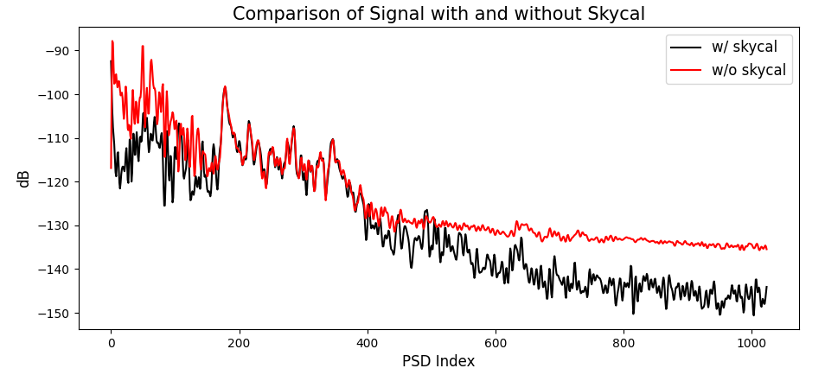
\includegraphics[width=1\columnwidth]{FIGURES/SkyCal.png}
\caption{Frequency domain radar trace (black), with sky calibration (red).  }
\end{figure}
\end{minipage}
}
\end{mysection}

\begin{mysection}{Automatic layer picking: Genetic Algorithm}
\vspace{-1cm}
\large{
\begin{itemize}
\item Sky calibration used to define solution space, shown in gray in Fig. 5
\item Genetic algorithm (GA) used as a first guess at snow-ground interface
\item Uses 6 features from each trace, in groups of 1000 traces (about 1 minute of data)
\item Output becomes training data for Neural Network
\end{itemize}

\begin{minipage}{1\columnwidth}
\begin{figure}
\centering
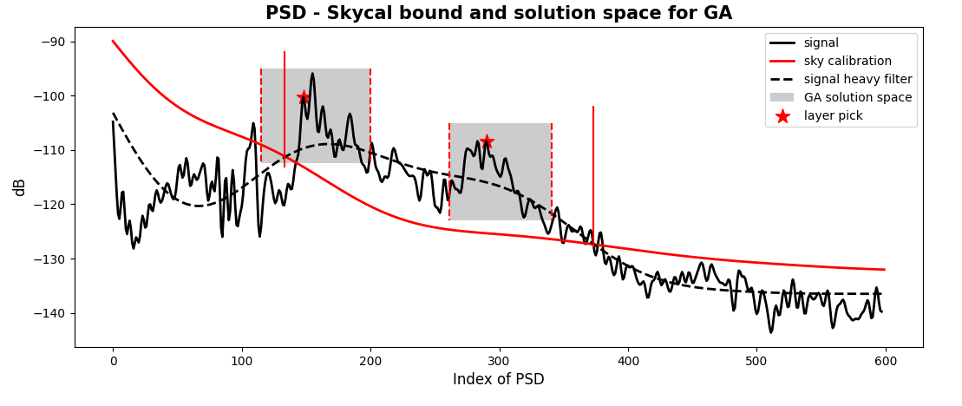
\includegraphics[width=1\columnwidth]{FIGURES/Bounds.png}
\caption{Sky calibration is used to define solution space for genetic algorithm.}
\end{figure}
\end{minipage}

}
\end{mysection}

\begin{mysection}{Automatic layer picking: Neural Network}
\vspace{-1cm}
\large{
\begin{itemize}
\item Similar to recognition of handwritten numbers
\item NN is a multilayer perceptron, has two hidden layer, uses 30 traces centered on trace to pick
\item Uses output of genetic algorithm to train, avoiding the need for manually picking layers in training data
\end{itemize}

%\begin{minipage}{0.5\columnwidth}
%\begin{figure}
%\centering
%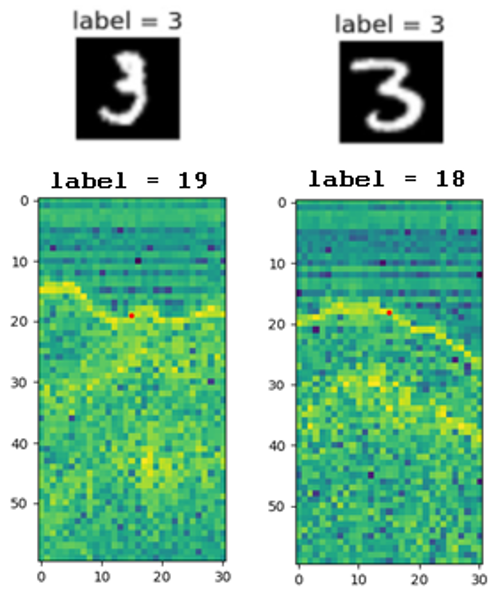
\includegraphics[width=1\columnwidth]{FIGURES/CNN.png}
%\caption{\small{}}
%\end{figure}
%\end{minipage}

\begin{minipage}{1\columnwidth}
\begin{figure}
\centering
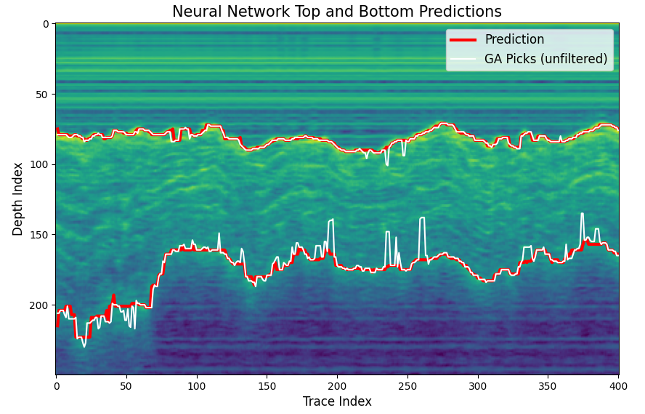
\includegraphics[width=1\columnwidth]{FIGURES/NeuralNetPicks.png}
\caption{Genetic algorithm picks (white), used as training for neural network (picks shown in red).}
\end{figure}
\end{minipage}

}
\end{mysection}

\begin{mysection}{Validation: Comparison to manual probe depth}
\vspace{-1cm}
\large{
\begin{itemize}
\item Comparisons made at 24 pits where radar drove same spiral coincident with manual probe measurements
\item Similar to previous studies \citep{McGrath:2019,Webb:2020}, manual probes are deeper, likely due to over probing
\item Comparison of mean depth across 24 pit sites, not used for training, shows good agreement (r=0.95, RMSE<5cm) with automatic picking
\end{itemize}

\begin{minipage}{1\columnwidth}
\begin{figure}
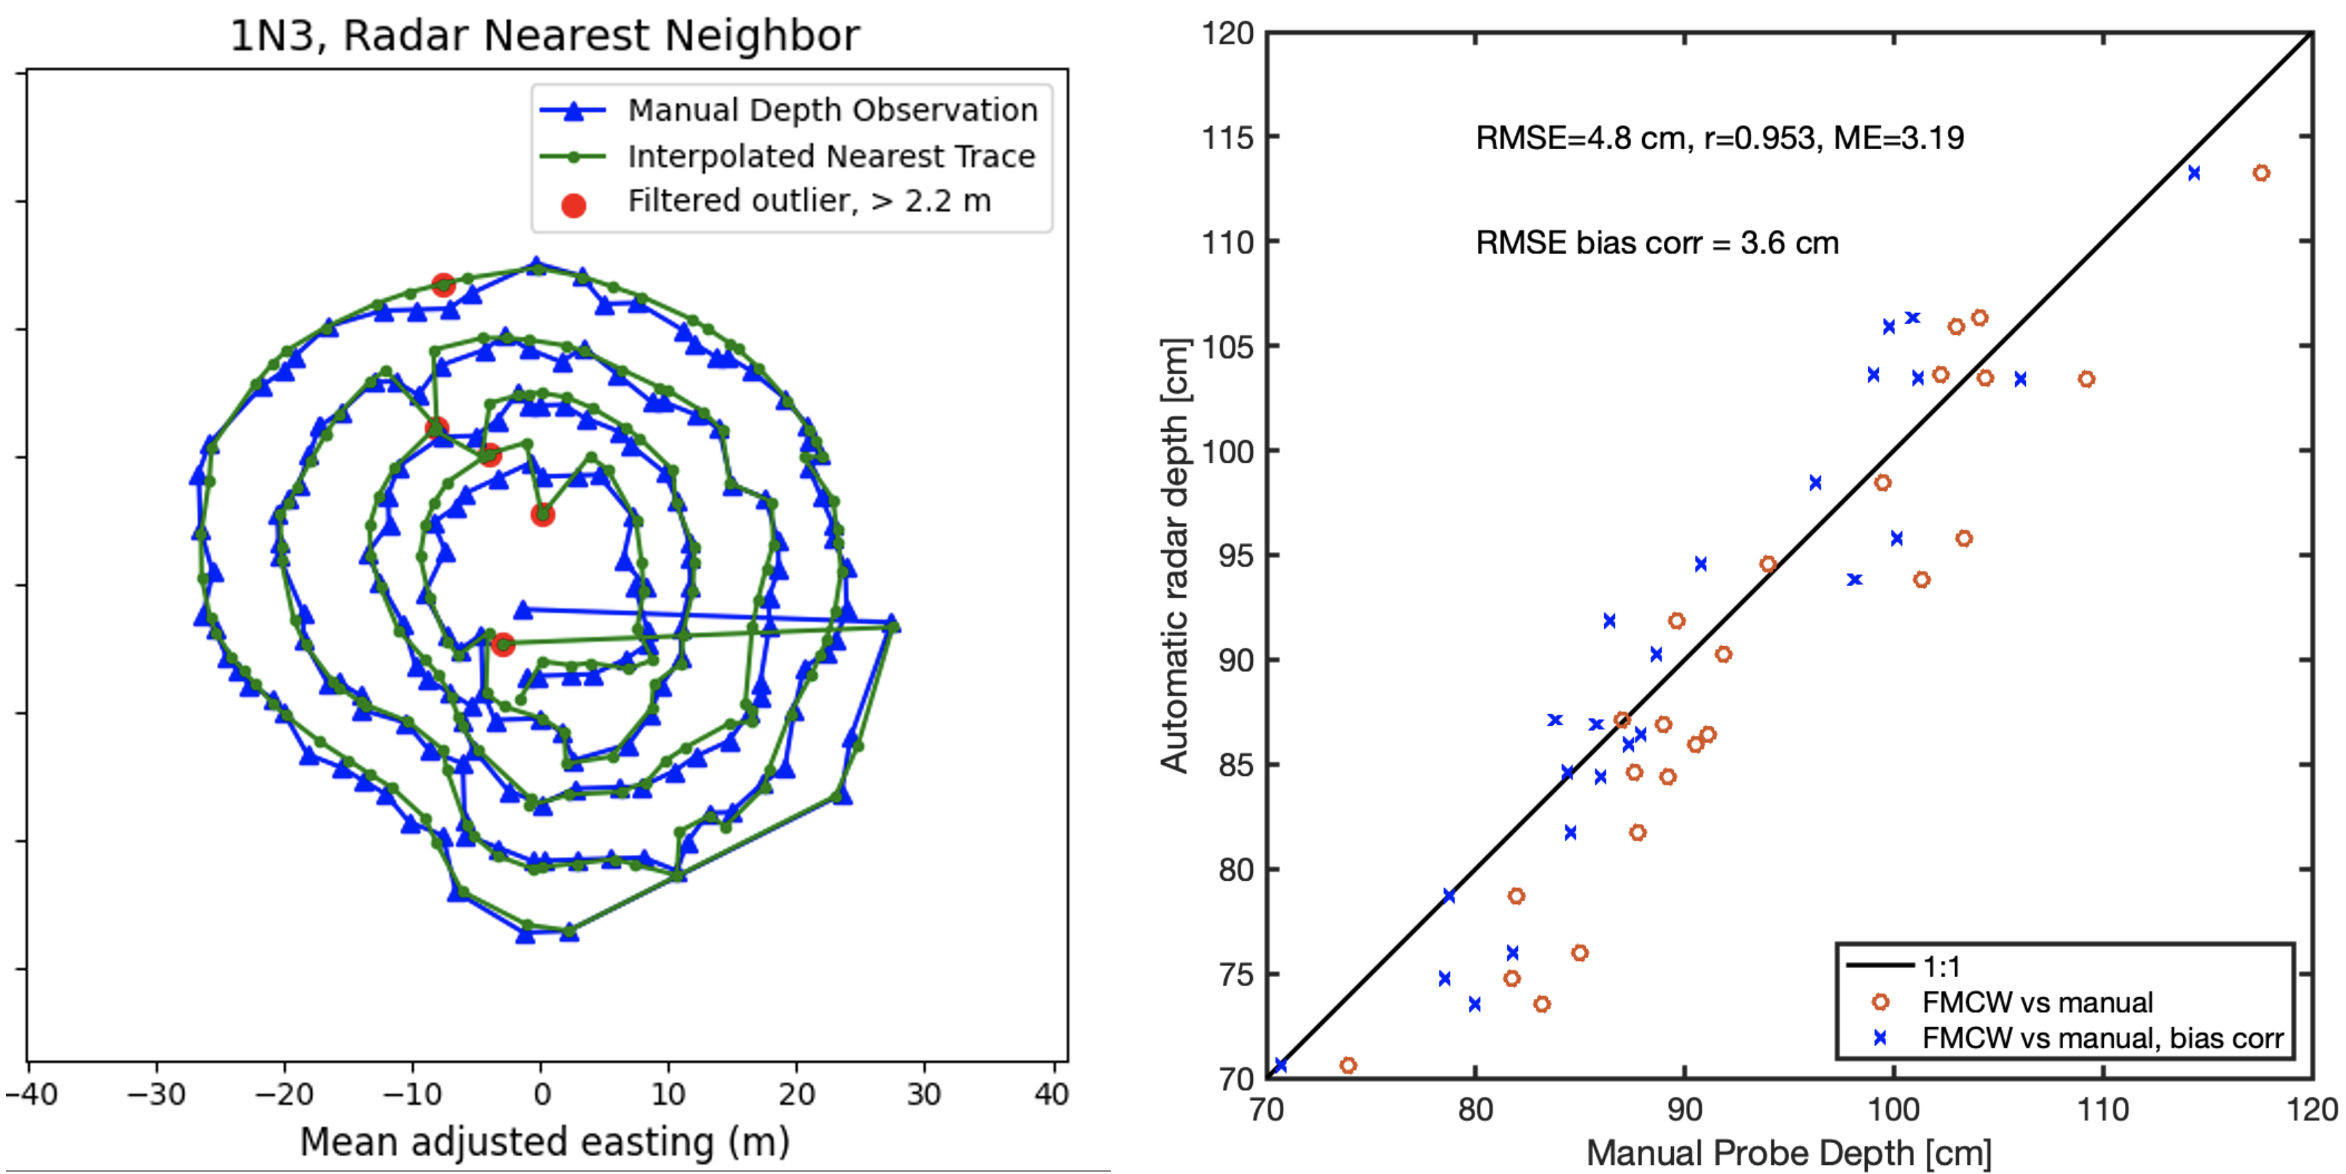
\includegraphics[width=1\columnwidth]{FIGURES/SpiralCompare.png}
\caption{Example spiral around snowpit, showing location of manual depth observations and radar transects (left), and a comparison of mean manual depth observations and automatic radar results at 24 test pits.}
\end{figure}
\end{minipage}

}
\end{mysection}

\begin{mysection}{Stratigraphy Information}
\vspace{-1cm}
\large{
\begin{itemize}
\item Stratigraphy can cause challenges for active and passive microwave retrievals of snow
\item Random forest used to classify radar profiles into high stratigraphy and low stratigraphy regions
\end{itemize}

\begin{minipage}{1\columnwidth}
\begin{figure}
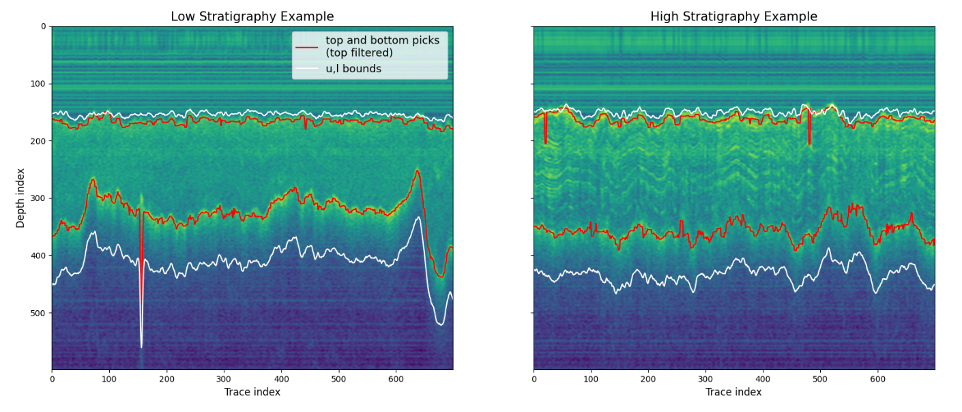
\includegraphics[width=1\columnwidth]{FIGURES/Stratigraphy.png}
\caption{Random forest classified radar transects as either low stratigraphy (left) or high stratigraphy (right).}
\end{figure}
\end{minipage}

}
\end{mysection}


%\begin{mysection}{Depth change and total depth, compared to in-situ observations}
%\vspace{-1cm}
%\large{
%\begin{itemize}
%\item 
%\end{itemize}
%
%\begin{minipage}{1\columnwidth}
%\begin{figure}
%\centering
%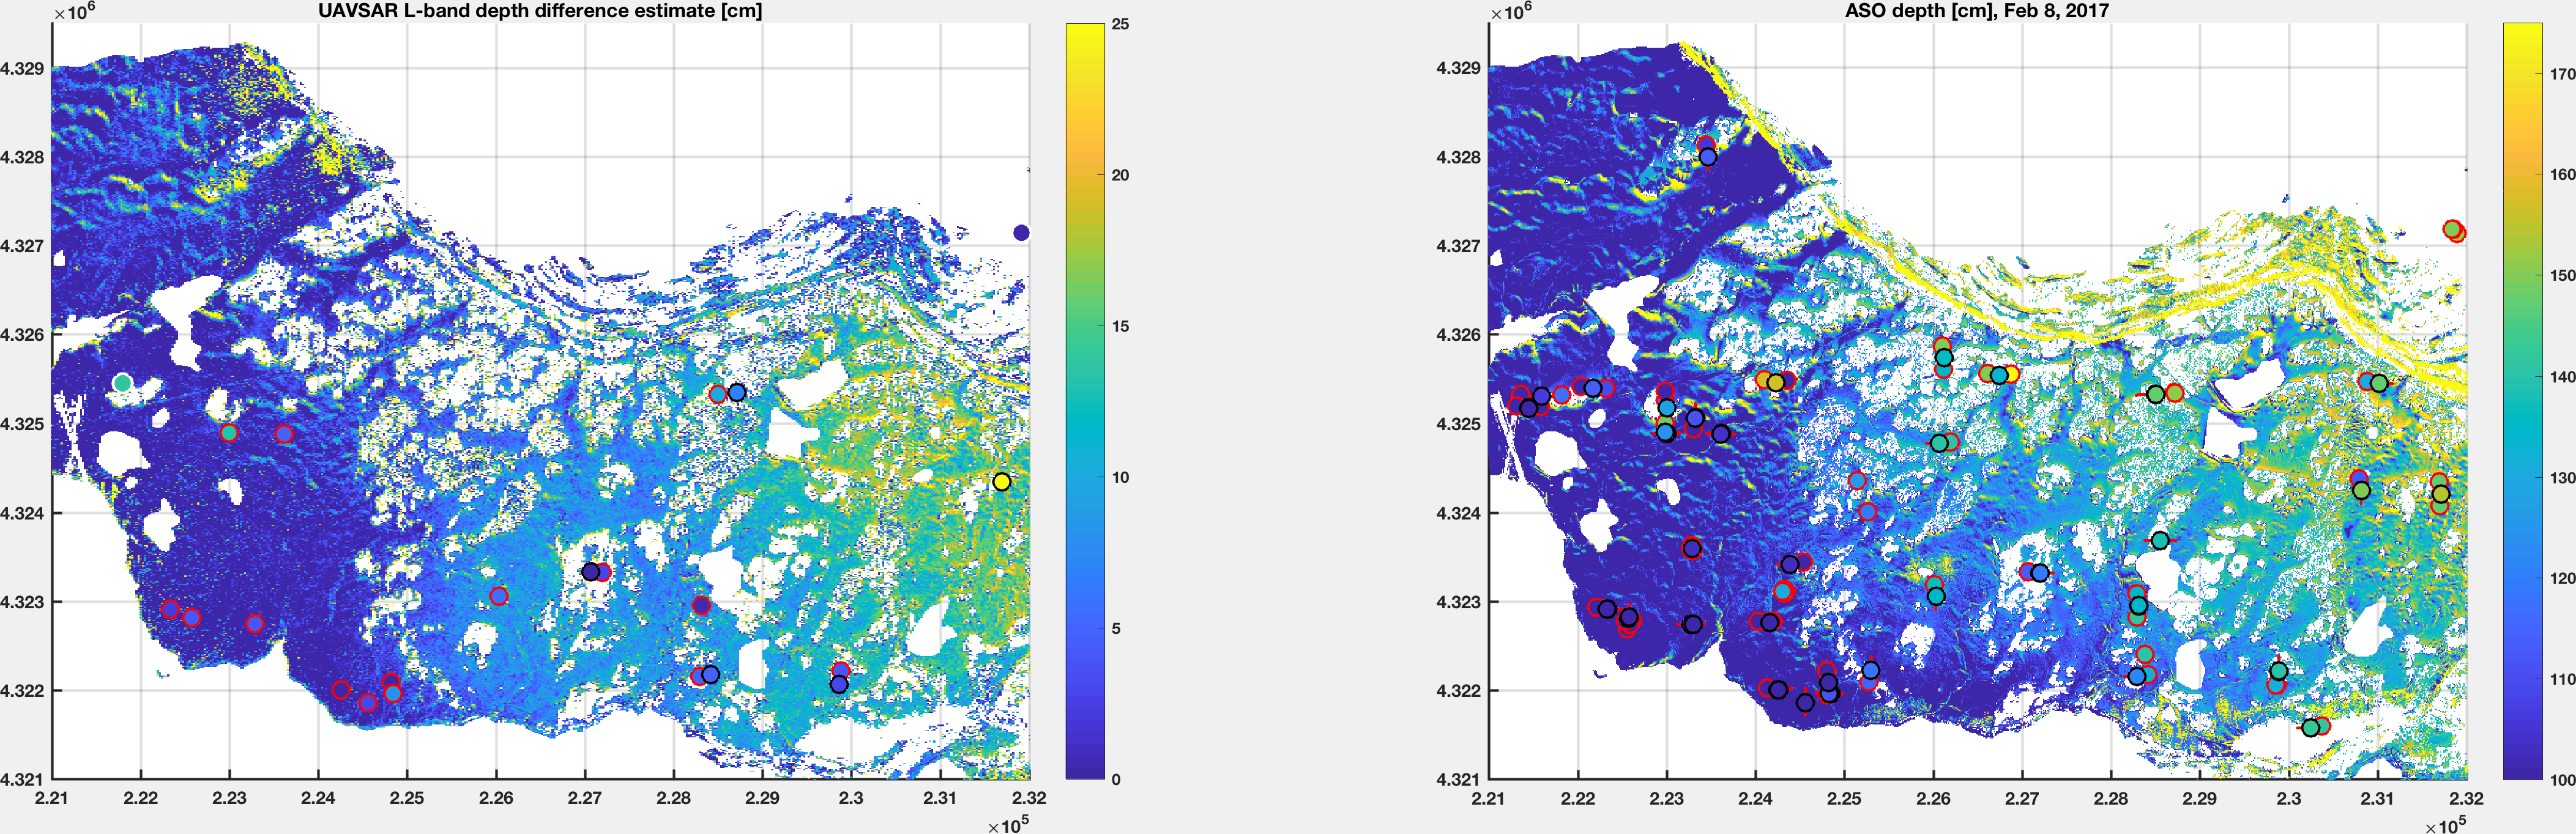
\includegraphics[width=1\columnwidth]{Fig8.png}
%\caption{\small{Left: InSAR depth estimate, with in-situ depth changes shown with filled circles.  Right: LiDAR snow depth, with in-situ depths shown with filled circles.}}
%\label{fig:InSAR_LiDAR_1km} 
%\end{figure}
%\end{minipage}
%
%}
%\end{mysection}
%\begin{mysection}{InSAR depth change at 1 km$^2$ scale}
%\vspace{-1cm}
%\large{
%\begin{itemize}
%\item 
%\end{itemize}
%
%\begin{minipage}{1\columnwidth}
%\begin{figure}
%\centering
%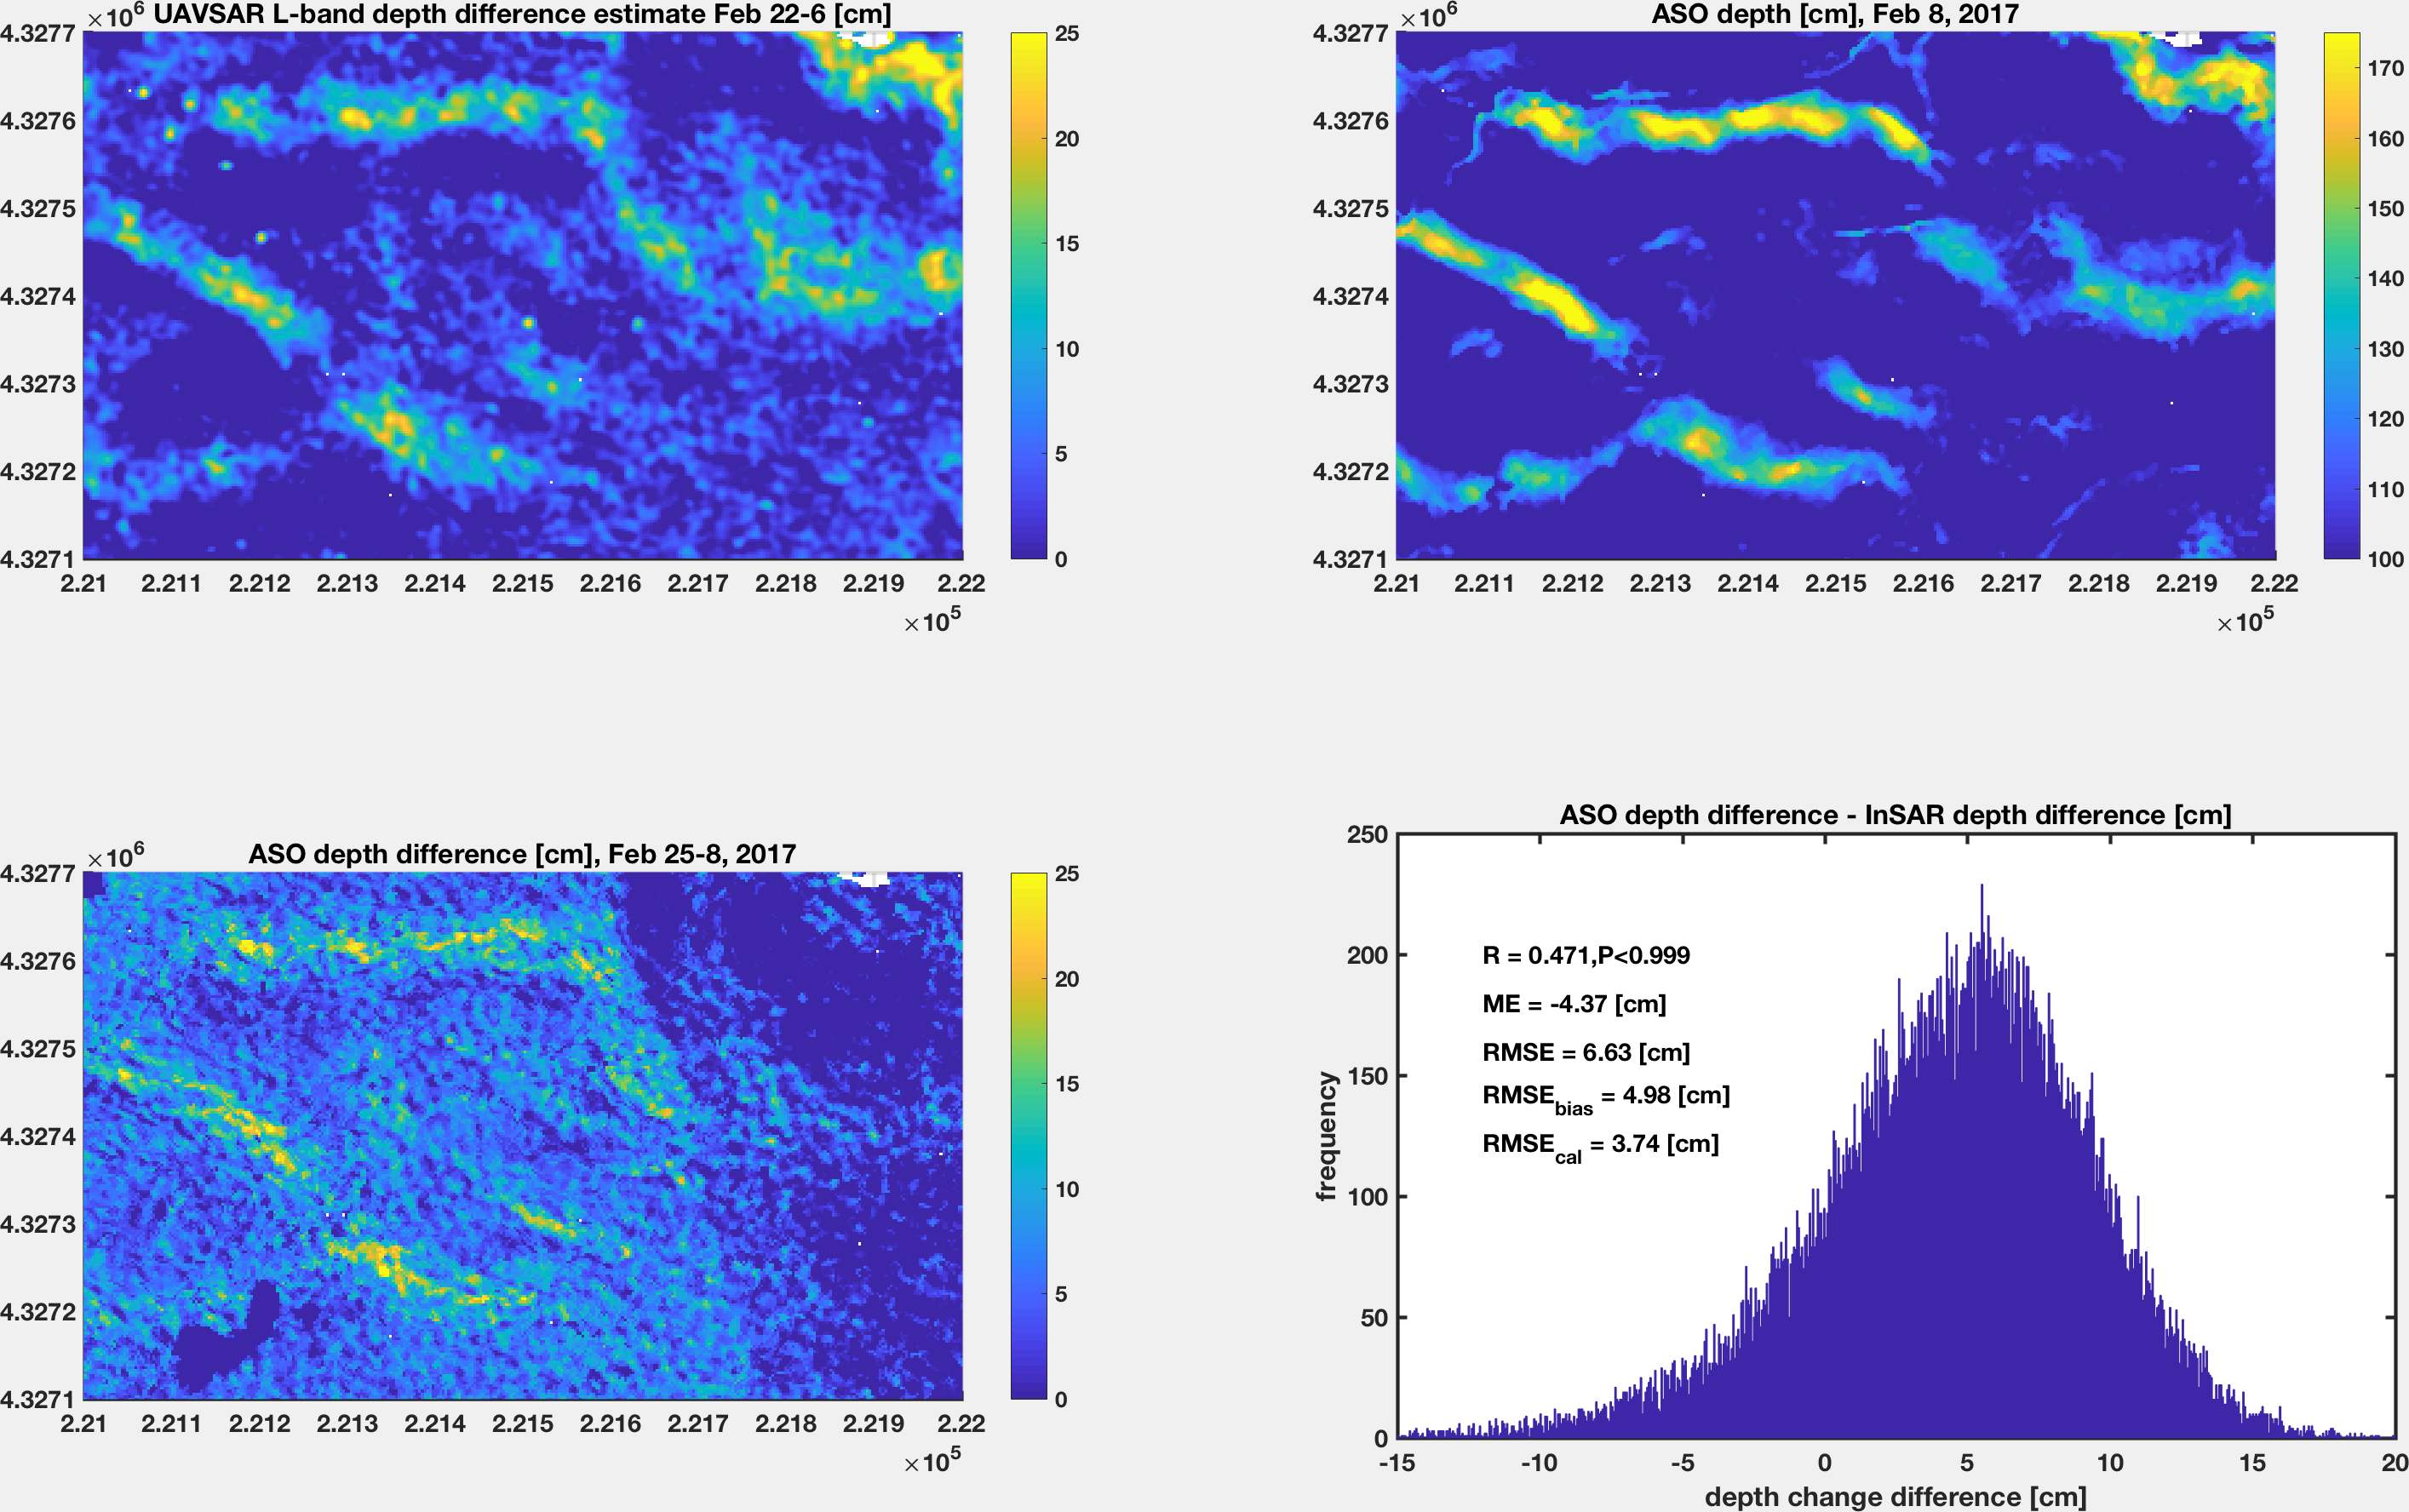
\includegraphics[width=1\columnwidth]{Fig9.png}
%\caption{\small{Top left: InSAR depth change retrieval. Top right: LiDAR snow depth.  Bottom left: LiDAR depth change.  Bottom right: histogram of LiDAR-InSAR depth change.}}
%\label{fig:InSAR_LiDAR_1km} 
%\end{figure}
%\end{minipage}

%}
%\end{mysection}


%\large{
%\begin{minipage}{0.6\columnwidth}
%\begin{figure}
%  \begin{center}
%   \includegraphics[width=1\columnwidth]{FMCWinsitu.pdf}
%   \caption{\small{Snowpit observations, In-situ reflectivity, FMCW profile, metal reflector exp}}
%   \label{fig:multiGPR} 
%  \end{center}
% \end{figure}
%\end{minipage}
%\begin{minipage}{0.35\columnwidth}
%\begin{figure}
%  \begin{center}
%   \includegraphics[width=1\columnwidth]{Reflectivity.png}
%   \caption{\small{In-situ reflectivity vs. FMCW backscatter}}
%   \label{fig:multiGPR} 
%  \end{center}
% \end{figure}
%\end{minipage}
%
%\begin{minipage}{0.4\columnwidth}
%\begin{figure}
%  \begin{center}
%   \includegraphics[width=1\columnwidth]{InSitu.png}
%   \caption{\small{In-situ dielectric constant}}
%   \label{fig:multiGPR} 
%  \end{center}
% \end{figure}
%\end{minipage}
%\begin{minipage}{0.3\columnwidth}
%\begin{figure}
%  \begin{center}
%   \includegraphics[width=1\columnwidth]{Layers.png}
%   \caption{\small{Arctic snow stratigraphy}}
%   \label{fig:multiGPR} 
%  \end{center}
% \end{figure}
%\end{minipage}
%\begin{minipage}{0.3\columnwidth}
%\begin{figure}
%  \begin{center}
%   \includegraphics[width=1\columnwidth]{LayerVar.png}
%   \caption{\small{Layer variation in three parallel trenches over 50cm}}
%   \label{fig:multiGPR} 
%  \end{center}
% \end{figure}
%\end{minipage}
%
%\begin{minipage}{0.65\columnwidth}
%\begin{itemize}
%\item Continuous reflections caused by density changes at layer boundaries
%\item Cause of reflections can be confirmed with metal reflection experiments
%\item Amplitude of reflection is a function of dielectric contrast
%\item Small scale variations in stratigraphy larger than variations in bulk properties
%\item Average reflectivity and average radar backscatter from layer boundaries highly correlated
%\end{itemize}
%\end{minipage}
%\begin{minipage}{0.3\columnwidth}
%\begin{figure}
%  \begin{center}
%   \includegraphics[width=1\columnwidth]{MuliGPR.pdf}
%   \caption{\small{Multi-channel radar for continuous density profiling}}
%   \label{fig:multiGPR} 
%  \end{center}
% \end{figure}
%\end{minipage}
%
%}
%\end{mysection}

%%% Conclusions %%%
%\begin{mysection}{Conclusions}
%\large{
%\begin{itemize}
%\item Variations below 500 m can be large, and high resolution observations at the km-scale are needed to understand and model snow distribution accurately
%\item High resolution (2cm vertical, 10cm horizontal) radar measurements produce detailed view of spatial distribution of depth, density, stratigraphy and density profiles at a resolution and scale not possible with traditional techniques.  
%\item Measurements at the km scale are quick and low cost, and bridge the gap between point observations and remote sensing and modeling pixel scales.
%\item Amplitude of reflections from layer boundaries are highly correlated with magnitude of density change, but require averaging many observations
%\item Multi-channel radar allows independent measurements of layer thickness and density
%\item Combining multi-channel radar with forward modeling = accurate profiles of density, layer boundaries, liquid water content 
%\end{itemize}
%
%\begin{minipage}{0.4\columnwidth}
%\begin{figure}
%  \begin{center}
%   \includegraphics[width=1\columnwidth]{DoubleRadar.jpg}
%   \label{fig:SMP_profile} 
%  \end{center}
% \end{figure}
%\end{minipage}
%\begin{minipage}{0.3\columnwidth}
%\begin{figure}
%  \begin{center}
%   \includegraphics[width=1\columnwidth]{HPAndyRadar.jpg}
%   \label{fig:SMP_profile} 
%  \end{center}
% \end{figure}
%\end{minipage}
%\begin{minipage}{0.3\columnwidth}
%\begin{figure}
%  \begin{center}
%   \includegraphics[width=1\columnwidth]{radar2.jpg}
%   \label{fig:SMP_profile} 
%  \end{center}
% \end{figure}
%\end{minipage}
%}
%\end{mysection}


\begin{mysection}{Acknowledgments}

\small{
This work was funded by the NASA Terrestrial Hydrology Program, grant \#NNX17AL61G and U.S. Army CRREL.  The authors thank all of the SnowEx 2020 Grand Mesa observers, without whom this work would not have been possible.

%\nocite{Deeb:2011,Engen:2004,Li:2017}

%\vspace{-2cm}

\bibliography{mypubs2}
}
\end{mysection}



\end{multicols}
  
%\begin{multicols}{2}
%\begin{mysection}{Km-scale profiles}
%\large{
%\begin{minipage}{0.6\columnwidth}
%\begin{figure}
%  \begin{center}
%\includegraphics[width=1\columnwidth]{SBB.png}
%\caption{\small{2-10 GHz FMCW radar measurements in the high alpine, Senator Beck Basin, CO.}}
%\label{SBB} 
%\end{center}
%\end{figure}
%\end{minipage}
%\begin{minipage}{0.3\columnwidth}
%\begin{figure}
%\begin{center}
%\includegraphics[width=1\columnwidth]{SBB2.pdf}
%\caption{\small{Map of radar profiles in Senator Beck Basin.}}
%\label{SBTOP} 
%\end{center}
%\end{figure}
%\end{minipage}
%
%\begin{figure}
%\includegraphics[width=0.95\columnwidth]{LiDAR-Scale-Resolution5.pdf}
%\caption{\small{Why high resolution matters: details at scales less than 500m are often complex, complicating ground-truth of remote sensing footprints at this scale.}}
%\label{fig:LiDARres} 
%\end{figure}
%}
%\end{mysection}
%\end{multicols}
\end{poster}

\end{document}

